\section{Design and Implementation}
\label{sec:implementation}

This section describes how \MP{} profiles different aspects of memory allocators, such as performance overhead, memory overhead, scalability issue, and application friendliness. It also describes some common issues, such as adapting to different allocators, and the performance issue of collecting data. 

\MP{} is implemented as a library that can be preloaded before a memory allocator, other libraries, and applications. Therefore, \MP{} is able to intercept memory allocations/deallocations, memory-related system calls, and synchronizations, in order to profile an allocator. That is, an allocator should utilize standard APIs in order to be profiled. For instance, the Linux allocator should invoke explicit POSIX-APIs for synchronizations, instead of some internal synchronization APIs. Fortunately, most allocators do not need any change or the recompilation for the profiling.    

\subsection{Adapting To Different Allocators}

\label{sec:understandingallocators}

As described above, one challenge is to adapt \MP{} to different allocators. \MP{} relies on a prerun program to understand the difference of different allocators, including the allocator's style (BiBOP-style versus sequential), class sizes, the threshold of separating small objects from large objects. These details will be employed to differentiate small objects from large objects (with different performance overhead), and to compute the memory overhead. Programmers could also provide these details explicitly, without resorting to the prerun program.  

In order to identify the style of allocator, the prerun routine will check whether two subsequent allocations with different sizes (apparently from different size classes) are allocated from the same page or not. If yes, then the allocator is a sequential-style allocator, which is similar to the default Linux allocator. Otherwise, we will check whether two subsequent allocations with the same size are allocated from the same page. If the answer to this question is yes, then the allocator is a BiBOP-style allocator. \MP{} only deals with sequential and BiBOP-style allocators, which covers most popular allocators.  

\begin{figure}[!ht]
\centering
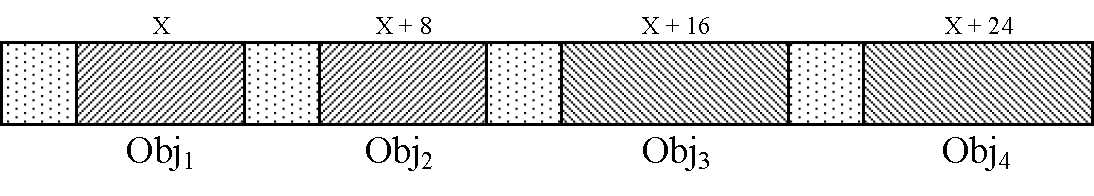
\includegraphics[width=5in]{figures/sequentialclasssize}
\caption{Determining the size class of a sequential allocator. \\The boxes with 10\% dotted pattern are the metadata, and the boxes with diagonal stripes\\ are actual heap objects. The number above every box is the size of the corresponding object. \label{fig:sizeclass}}
\end{figure}

The second step is to identify various size classes. The prerun routine begins by allocating an object of 8 bytes, and continues to allocate additional objects using a stride increase of 8 bytes each time. The determination of size classes depends on the style of an allocator. For BiBOP-style allocators, an allocation with a different size class will be satisfied from a different bag, locating in a different page. For sequential allocators, such as the Linux allocator, the distance between two  contiguously-allocated objects (with distinct sizes) is utilized to determine the size class. As shown in Fig.~\ref{fig:sizeclass}, since the distance of $Obj_1$ and $Obj_2$ is the same as the distance of $Obj_2$ and $Obj_3$, then $obj_1$ and $obj_2$ belong to the same size class. For the same reason, we could determine that $Obj_3$ belongs to a different size class.  

The threshold for big objects are typically detected by checking whether there is an explicit \texttt{mmap} system calls upon the allocation. Typically, most allocators utilize a direct \texttt{mmap} system call to satisfy the allocation for a big object. However, this threshold requires the manual confirmation. 
% , and observing whether a significant address difference exists between the placement of these objects. 

%Open BSD's allocator ``reverse aligns'' objects that are between 2Kb and 4Kb in size. The allocator aligns the objects last byte to the end of the page in which it resides, so that the object starting byte is somewhere in the middle. The prerun would see the address change and believe it has found a new class size. Open BSD provides a flag to turn this behavior off, however this is one example of the challenges of making the profiler general purpose.

%There are many challenges in searching for metadata. Different allocators employ completely different methods in storing metadata for it's internal use. There are a number of ways we attempt to get metadata size for each object. For a bibop allocator, it's metadata has a good chance of being located in a private memory region returned from mmap. The prerun detects the mmap and checks to see if it was used to fulfill a memory request. If it wasn't we will search it for metadata. The prerun library utilizes the /proc/pid/pagemap file to identify the virtual pages which are backed by physical frames. The prerun searches the entire mmap region for physically backed virtual pages, remembering their page numbers in relation to the mmap region starting address. Finally, the prerun counts the number of non-zero bytes on all physically-backed virtual pages, using the minimum of all these values as an estimated metadata size. This method works with the assumption that the bibop-style allocator \emph{is} placing it's metadata in mmap memory. One of the allocators we tested, Dieharder, does mmap memory that was not used for allocations nor metadata, however the prerun includes these regions in it's search for metadata incorrectly. Additionally, the actual metadata is interpreted differently for different allocators. One allocator can store primitive data types in it's metadata, while another allocator uses bitmaps or byte values that have specific meaning only to that allocator. The numerous ways of storing and interpreting metadata is a huge challenge for us.
		
%Another huge challenge in the profiler is globally storing data that is thread specific in a way that is quickly accessed and synchronized between threads. There's no getting around all threads needing to access some type of global data. Doing this efficiently is a priority for the profiler. Detecting memory blowup requires the allocating thread to be aware of other threads free object status. An internal global free list of objects has too much contention from threads simultaneously inserting, deleting, and searching the free list. We employ a semi-thread local approach. Each thread has a thread local count of free objects (by class size for bibop) and the profiler maintains one global count (again by class size for bibop). When a thread allocates, there are three possibilities that we check in determining memory blowup, always starting with the thread checking it's thread local free count. If the thread has free objects it can reuse, the profiler assumes that the thread will reuse one of it's free objects, and decrements its local and global counter. If the thread does not have free objects, it checks to see if there are free objects globally. If there are, the profiler accounts for that one occurrence of memory blowup and decrements the global counter. The last situation is that the thread does not have any free objects, and the global counter is at zero. There is no memory blowup in this situation. The global counter is synchronized using atomic accesses. This is accurate and fast method the profiler uses in detecting memory blowup. Balancing the profiler with accurate synchronized global data and performance is a huge challenge.

\subsection{Profiling Performance Overhead}

\label{sec:performanceimplement}

\MP{} profiles the performance overhead of every allocation and deallocation, as discussed in Section~\ref{sec:performanceimplement}. It also utilizes the PMUs to collect hardware events, such as cache misses, page faults, TLB misses, and instructions. For allocations, since each allocator has different execution paths for different scenarios, such as new or re-used allocation, small or big objects, \MP{} further collects the information for each scenario. The differentiation is mandatory to identify an issue inside a specific scenario. For instance, even if the average runtime of every allocation is normal, the allocator may still have an issue in dealing with one specific scenario, such as new allocation. \todo{Do we have some examples?} For deallocations, \MP{} tracks the data for small and big objects, due to the same reason. For instance, DieHarder has an issue for deallocating small objects, but it has the normal performance for deallocations of big objects.  

\MP{} easily differentiates large objects from small objects based on the threshold,  as described in Section~\ref{sec:understandingallocators}. In order to differentiate a new object from a re-used object, \MP{} utilizes a global hash map to track the status of each object. An object not in the hashmap is treated as a new object. 

%how each allocator differs with regard to allocation efficiency when reusing a previously freed object versus a new one. Timestamps taken both before and after each such execution pathway are compared in order to determine the total number of cycles spent within each path.

%We differentiate between used and new objects differently for BiBOP-style allocators and bump-pointer-based ones. For the former, counter arrays are used to track the number of free objects for each class size used by the allocator. In this way, if the given class size free-object-counter is non-zero, we will count the executed cycles toward the ``reused object'' pathway. Similarly for bump-pointer-based allocators, a simple running total is maintained for freed objects, and this total is compared to the size of the current allocation request.

\subsection{Profiling Memory Overhead}
\MP{} profiles the maximum memory data, including real memory usage, real allocated memory, and total memory. Real memory usage is the amount of memory actually requested  by the application, where real allocated memory is the sum of real memory usage and internal fragmentation caused by size-class based allocation. For example, if an application requests the memory by \texttt{malloc(454)}, then real memory usage is incremented by $454$, but real allocated memory will be incremented by $512$ (when the corresponding size class is $512$ bytes). For this case, total memory will be  be incremented by the page size (e.g., 4096 bytes), provided that the page was previously unused. 
%In order to track the maximum memory data, \MP{} will update the global data 

\MP{} reports different types of memory overhead when the total memory usage reaches its maximum value, such as internal fragmentation, external fragmentation, and memory blowup. It could also reports the available memory of each size class and the available memory for big objects.  Therefore, it helps programmers to pinpoint the memory overhead issue of a specific allocator. For instance, if the memory overhead mainly comes from the internal fragmentation, then the allocator should utilize more fine-grained size class. If the memory overhead mainly comes from the memory blowup, the allocator may require to adjust its synchronization frequency or take a more aggressive method for its synchronization~\cite{DBLP:conf/iwmm/LiLD19}. 

In order to track different types of memory overhead, \MP{} typically increments the corresponding counter upon each allocation and decrements it upon each deallocation. \MP{} utilizes a global hash table to track the status information of each object, which is the same table for determining new or re-used object. Therefore, \MP{} could adjust corresponding counters upon deallocation. 

 In order to reduce the contention issue, \MP{} typically maintains a per-thread counter for internal fragmentation, and updates the global counter periodically.  Based on the definition, external fragmentation occurs when an allocator has sufficient memory but in a non-continuous way. Therefore, \MP{} keeps a global counter for the available memory, so that it could determine whether an allocation causes the external fragmentation issue or not.  The counter for the memory blowup will be incremented, if the current per-thread heap has no freed objects but there exit freed objects with the requested size class in other per-thread heaps. Therefore, \MP{} maintains a global counter for each size class. 

% Upon an allocation request, if the current thread does not possess any freed objects of the given size class -- but if the global counter does -- we record this event as an allocation responsible for increasing the allocator's memory blowup.

  
  \todo{Based on the definitions of memory blowup and external fragmentation, an allocation will be counted as a memory blowup if there exists freed objects with the same size class. However, it is difficult to evaluate the external fragmentation. For instance, if freed objects with smaller class sizes exist, with the total size larger than the requested size, then the current allocation should be counted as external fragmentation. However, if freed objects with larger class sizes exist, it should not count as external fragmentation. But the overhead is caused by the issue of size class or without-splitting. Maybe we should make it clear in Section 3.3. }     
 

\subsection{Profiling Scalability}
\MP{} also reports a variety of metrics to  evaluate the scalability of a memory allocator. As described in Section~\ref{sec:scaleidea}, \MP{} evaluates the scalability for both user space and kernel space. 

For user-space scalability, \MP{} focuses on different types of locks, such as mutex locks, spin locks, and try locks. For each lock, \MP{} collects the number of acquisitions, the runtime of each acquisition (with RDTSC timestamp), the number of contentions, and the number of maximum contending threads. \todo{\MP{} dynamically maintains the contention state of each lock. Upon the acquisition, \MP{}  increments the contention threads of the corresponding lock, which will be decremented upon the release of this lock.} 

For the kernel-space scalability, \MP{} focuses on memory-related system calls inside the allocation and deallocation, including \texttt{mmap}, \texttt{munmap}, \texttt{mremap}, \texttt{sbrk}, \texttt{madvise}, and \texttt{mprotect}. The system calls outside memory management operations are excluded, since they are specific to applications. \MP{} collects the runtime of each invocation, and the number of invocations for each system call. In fact, the simple data could actually uncover  serious scalability issues of a memory allocator. For instance, the Linux allocator of \texttt{glibc-2.21} slows down an application by 40\%, which can be uncovered by the excessive number of \texttt{madvise} system calls and a higher runtime for the corresponding \texttt{mmap} and \texttt{mprotect} system call.   

\todo{We should collect the data for each type of allocations and deallocations, similar to the overhead. }


\subsection{Application Friendliness}
\label{sec:profilefriendliness}

\MP{} also reports whether an allocator is friendly to a specific application. More specifically, \MP{} focuses on the following parameters, including (1)~the average cache line utilization; (2)~the average page utilization; (3)~the number of cache misses caused by conflicting misses. As discussed in Section~\ref{sec:friendliness}, a user-friendly allocator should have  high cache-line and page utilization rates, but with a low number of conflicting cache misses.  

\MP{} employs the PMU-based sampling to track the average cache utilize and page utilization. Basically, \MP{} samples memory accesses periodically, with a default sampling period of 5,000. Upon every sampled event, \MP{} collects the number of used bytes for the current cache line and the current page, and also increments the number of sampled cache lines and pages. In the end, \MP{} computes the utilization rate  based on a simple division. For cache utilization rate, the dividend is the total number of used bytes, and the divisor is the the total number of bytes for these cache lines. The page utilization rate is computed similarly. 

However, the challenge is to quickly locate the  metadata for each cache line and each page, since the metadata should be updated upon every allocation and deallocation, and upon every sampled event. During its implementation, \MP{} has tried multiple mechanisms. First, \MP{} designed a red-black tree to hold memory mappings of the heap, and then stored the address of corresponding metadata on the tree node. This mechanism was found to be not efficient, since some allocators (e.g., OpenBSD) includes thousands of mappings, which may introduce tens of comparisons unfortunately. Second, \MP{} utilized a hash map to store the memory mappings. But it is difficult to decide the number of buckets for the hash table. For instance, if the number of buckets is designed to be small,  a large number of conflicts can be introduced, with significant performance overhead by traversing the link list.  Finally, \MP{} designs a fast lookup mechanism by taking advantage of the vast address space of 64-bits machines, where the detailed design is discussed as follows. 

% Based on our observation, all allocators invoke either \texttt{sbrk} or \texttt{mmap} system calls to obtain the memory from the underlying OS. The address range returned from \texttt{sbrk} is generally lower than 4G, while the range returned by \texttt{mmap} is typically less than 128TB. 
%Given that modern processors typically support 48 bits address space (256 TB), \MP{} employs the last TB (between 255TB and 256TB) of address space to store the meta data of object, with the design illustrated in Figure~\ref{fig:lookup}. 

\textbf{Three-Level Fast Lookup Mechanism:} \MP{} designs a three-level lookup mechanism as illustrated in Fig.~\ref{fig:lookup}, borrowing the idea of multi-level page table design of OS. Basically, a ``MB Mapping'' will be the first level, where the index can be computed simply by dividing an address with 1 MB. Each entry of this MB mapping points to all possible pages inside the current 1-megabyte memory. Since one MB memory will have at most 256 pages, with the size of 4KB for each page, each MB entry points to 256 page entries. Similarly, each page entry has the information about used bytes in this page and has a pointer pointing to 64 possible cache entries inside. Based on this design, it takes two steps to get the used bytes for a page, and takes three steps to get the used bytes for the current cache line. Therefore, it has the $\mathcal{O}(1)$ 
complexity to obtain the metadata.  
          
\begin{figure*}[!ht]
\centering
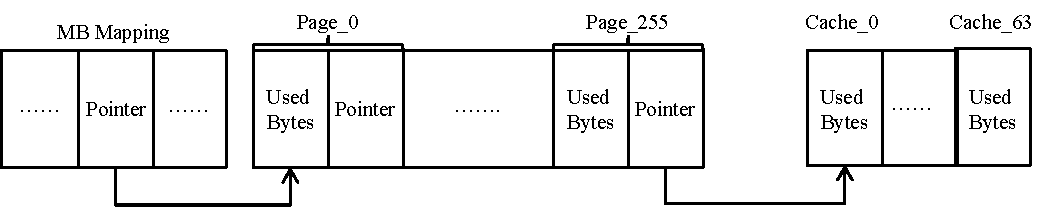
\includegraphics[width=5.5in]{figures/lookup2}
\caption{Three-level Lookup Mechanism.\label{fig:lookup}}
\end{figure*}

Note that this design is also efficient in memory consumption. If a range of addresses are not used, then there is no need to allocate physical memory for the corresponding page entries and cache entries. This design is able to adapt to different allocators, where memory mappings of a heap is varied from a few to hundreds of thousands, and these mappings can be scattered along the whole address space of a process. To track valid memory mappings dynamically, \MP{} intercepts memory related system calls inside allocations/deallocations, such as \texttt{sbrk}, \texttt{mmap}, \texttt{munmap}, \texttt{mremap}. 